\section{Benchmark}

All benchmarks were compiled using \texttt{g++} 13.3.0 and executed on an Intel Core i5 2.60\,GHz CPU. One of the test sets uses data from the US Road System, available at \url{https://www.diag.uniroma1.it/~challenge9/download.shtml}.

\subsection{Performance evaluation}

To assess the performance of the various priority queues, several scenarios were considered:

\begin{itemize}
  \item \textbf{Universe size scaling:} Time and memory usage were measured for different integer key universe sizes, using 1,000,000 randomized \texttt{push} and \texttt{pop} operations. This test was designed to evaluate how integer-based priority queues scale with increasing key space.

  \item \textbf{Queue size scaling:} To examine the effect of queue size, a fixed universe size of $2^{25}$ was used. For each test, a bulk of elements was inserted using \texttt{push} operations, followed by their removal using \texttt{pop}. Time and memory usage were measured separately for both phases.

  \item \textbf{String key performance:} (General-purpose queues only) This test assessed time usage when operating on long random string keys (1024 characters), with varying queue sizes. The goal was to evaluate the impact of costly key comparisons on overall performance.

  \item \textbf{Practical application:} (General-purpose queues only) Each queue was integrated into Dijkstra's shortest path algorithm~\cite{dijkstra1959note} and tested on real-world graphs from the 9th DIMACS Implementation Challenge. The following datasets of various sizes from the US Road System were used to compare real-world runtime performance:
  
  \begin{itemize}
  \item \textbf{USA-road-d.NY.gr}: 264,346 nodes, 730,100 edges, 13.77 MB
  \item \textbf{USA-road-d.FLA.gr}: 1,070,376 nodes, 2,687,902 edges, 53.07 MB
  \item \textbf{USA-road-d.CAL.gr}: 1,890,815 nodes, 4,630,444 edges, 95.41 MB
  \item \textbf{USA-road-d.W.gr}: 6,262,104 nodes, 15,119,284 edges, 325.84 MB
  \item \textbf{USA-road-d.CTR.gr}: 14,081,816 nodes, 33,866,826 edges, 756.36 MB
  \item \textbf{USA-road-d.USA.gr}: 23,947,347 nodes, 57,708,624 edges, 1322.82 MB
\end{itemize}
\end{itemize}

Below we provide results of the performance test scenarios mentioned. In all cases we also provide a baseline implementation from the C++ STL Library for comparison. The Figure~\ref{fig:structure_legend} presents the common legend for all plots.

\begin{figure}[H]
    \centering
    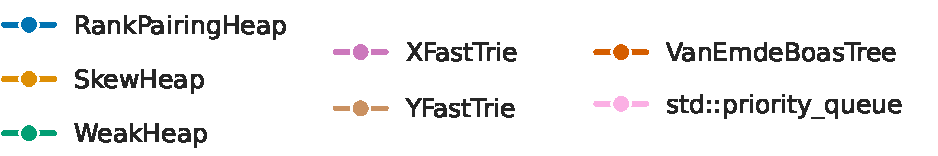
\includegraphics[width=0.9\textwidth]{figures/plots/legend.pdf}
    \caption{Legend assigning colors to priority queue implementations.}
    \label{fig:structure_legend}
\end{figure}

\begin{figure}[H]
    \centering
    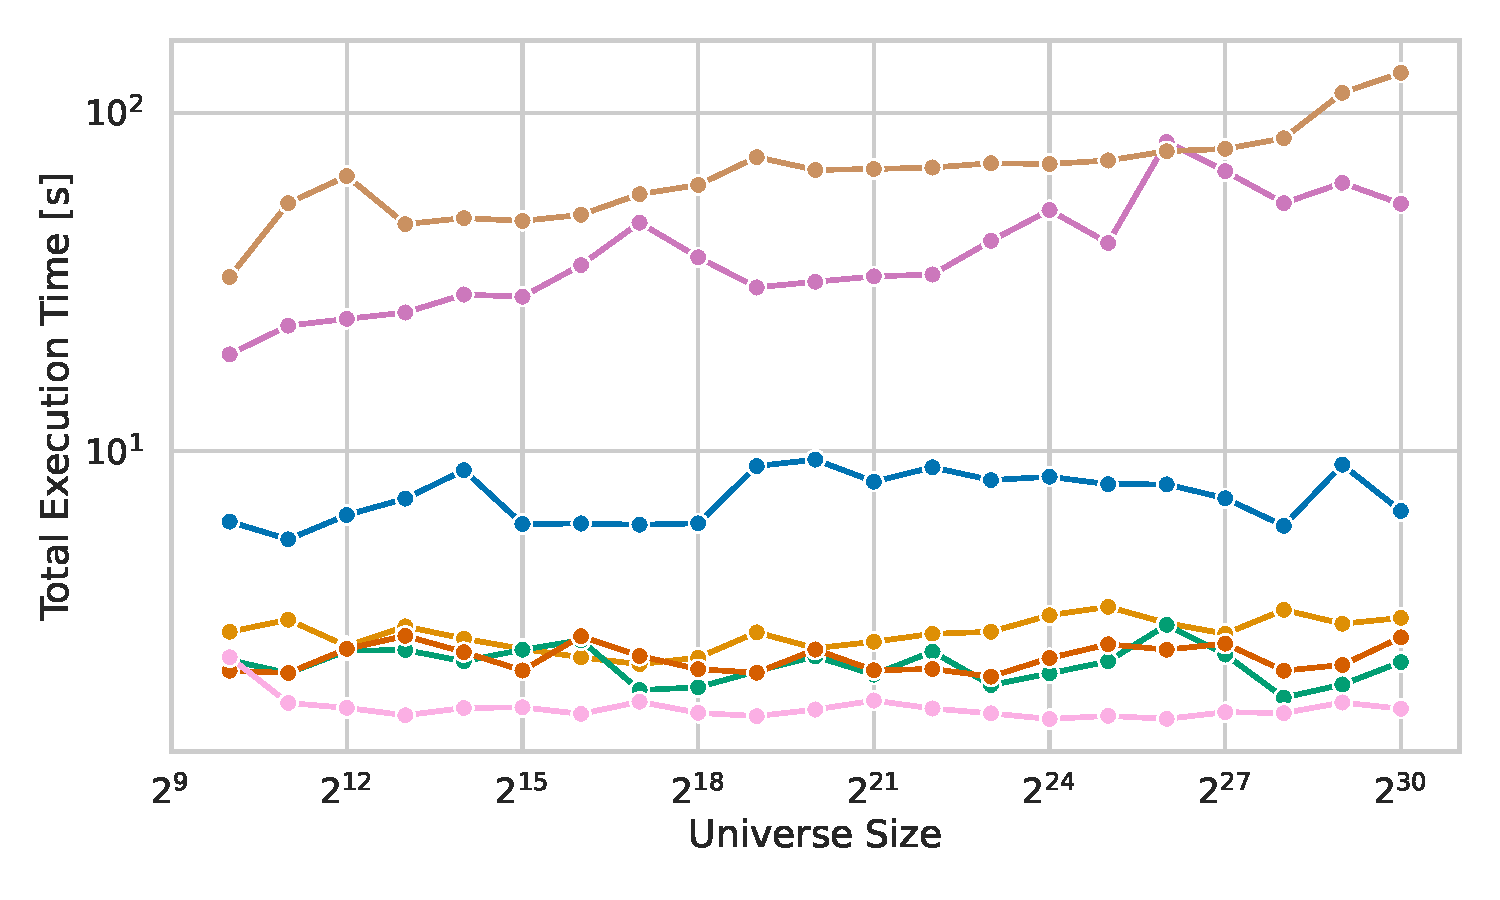
\includegraphics[width=1.0\textwidth]{figures/plots/plot_universe_vs_time.pdf}
    \caption{Total execution time vs. universe size.}
    \label{fig:Xfast_Yfast_performance}
\end{figure}

\begin{figure}[H]
    \centering
    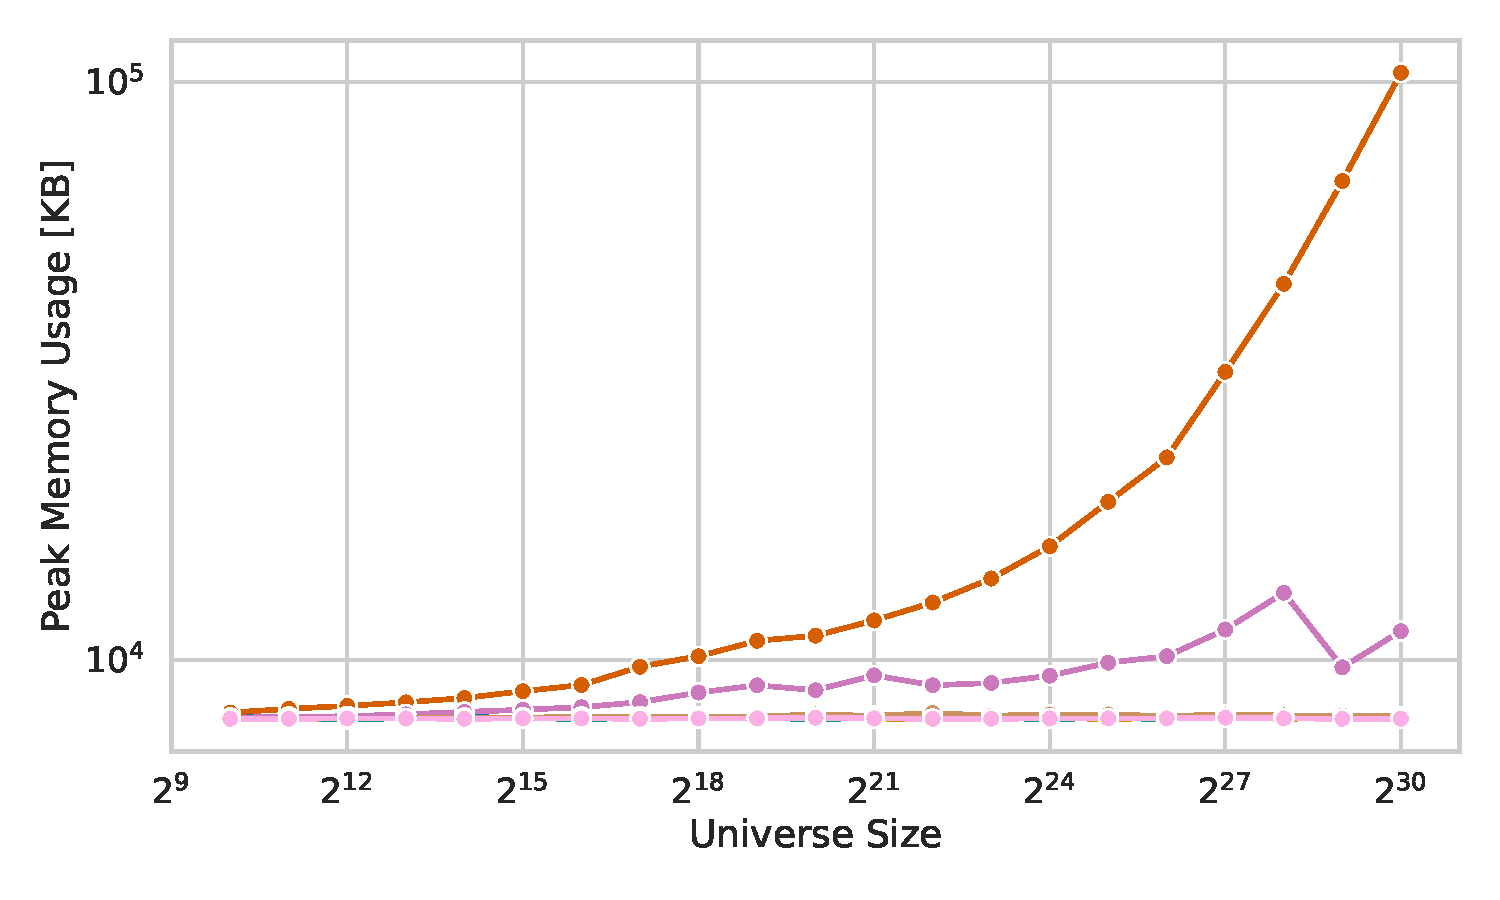
\includegraphics[width=1.0\textwidth]{figures/plots/plot_universe_vs_memory.pdf}
    \caption{Memory usage vs. universe size.}
    \label{fig:vEB_memory}
\end{figure}

\begin{figure}[H]
    \centering
    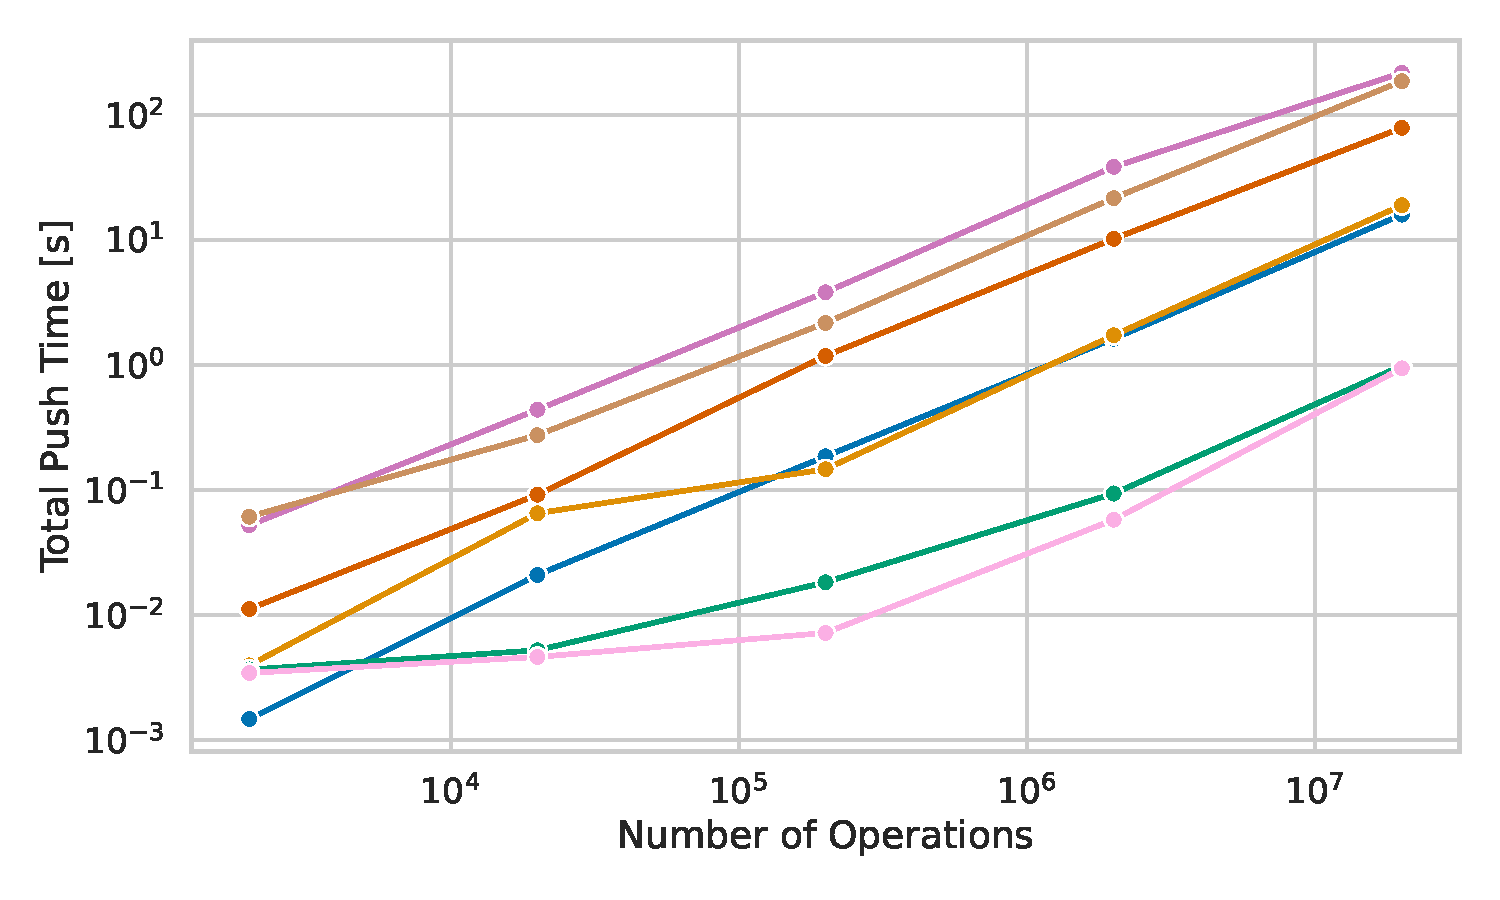
\includegraphics[width=1.0\textwidth]{figures/plots/plot_bulk_push.pdf}
    \caption{Push execution time vs. number of operations.}
\end{figure}

\begin{figure}[H]
    \centering
    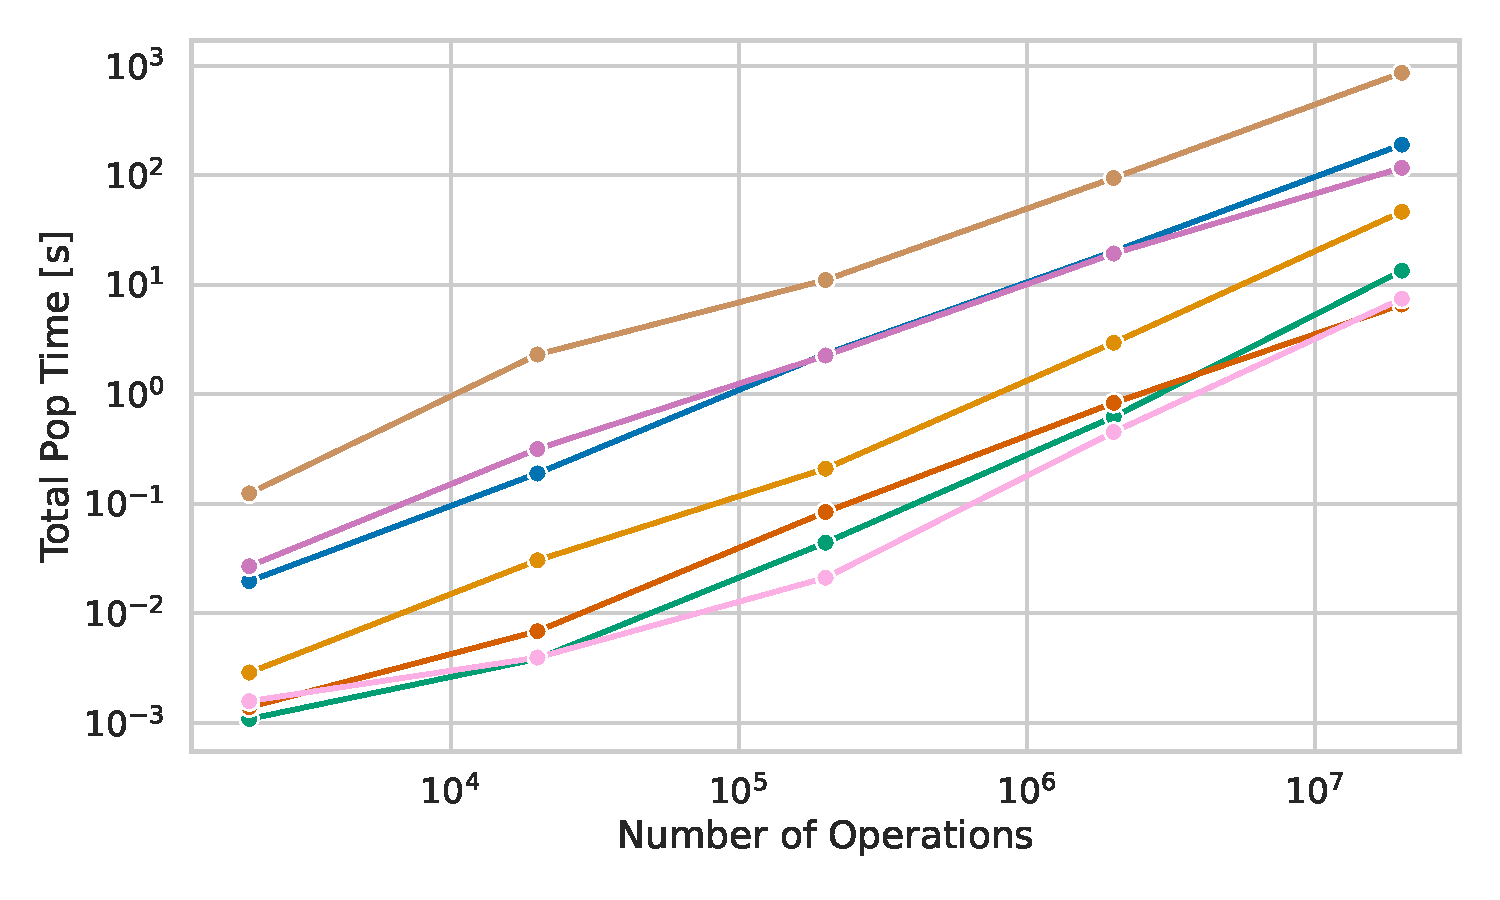
\includegraphics[width=1.0\textwidth]{figures/plots/plot_bulk_pop.pdf}
    \caption{Pop execution time vs. number of operations.}
\end{figure}

\begin{figure}[H]
    \centering
    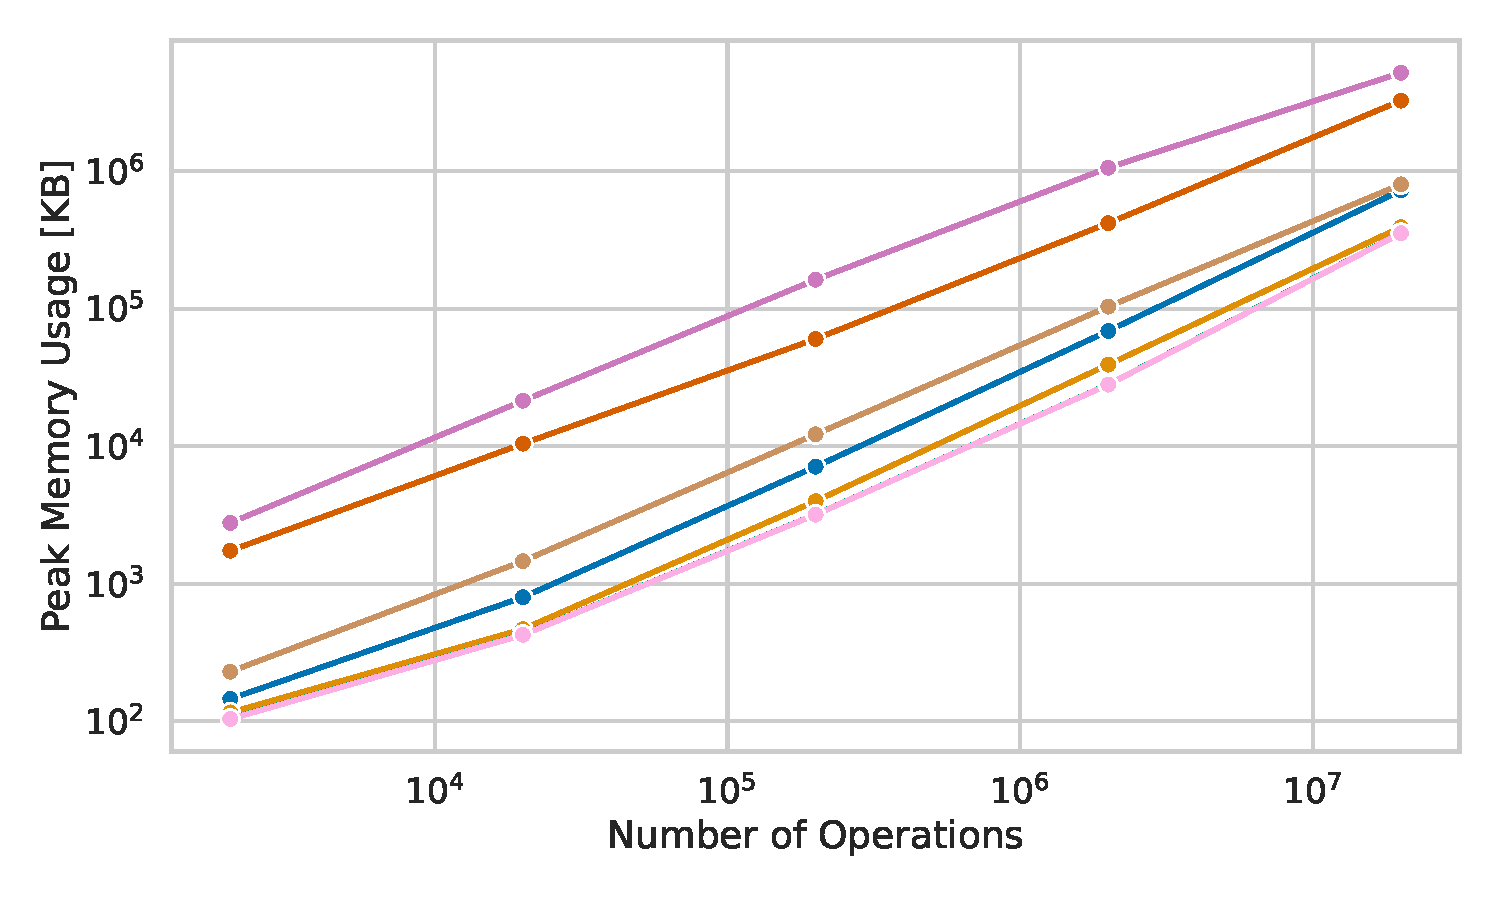
\includegraphics[width=1.0\textwidth]{figures/plots/plot_bulk_memory.pdf}
    \caption{Memory usage vs. number of operations.}
\end{figure}

\begin{figure}[H]
    \centering
    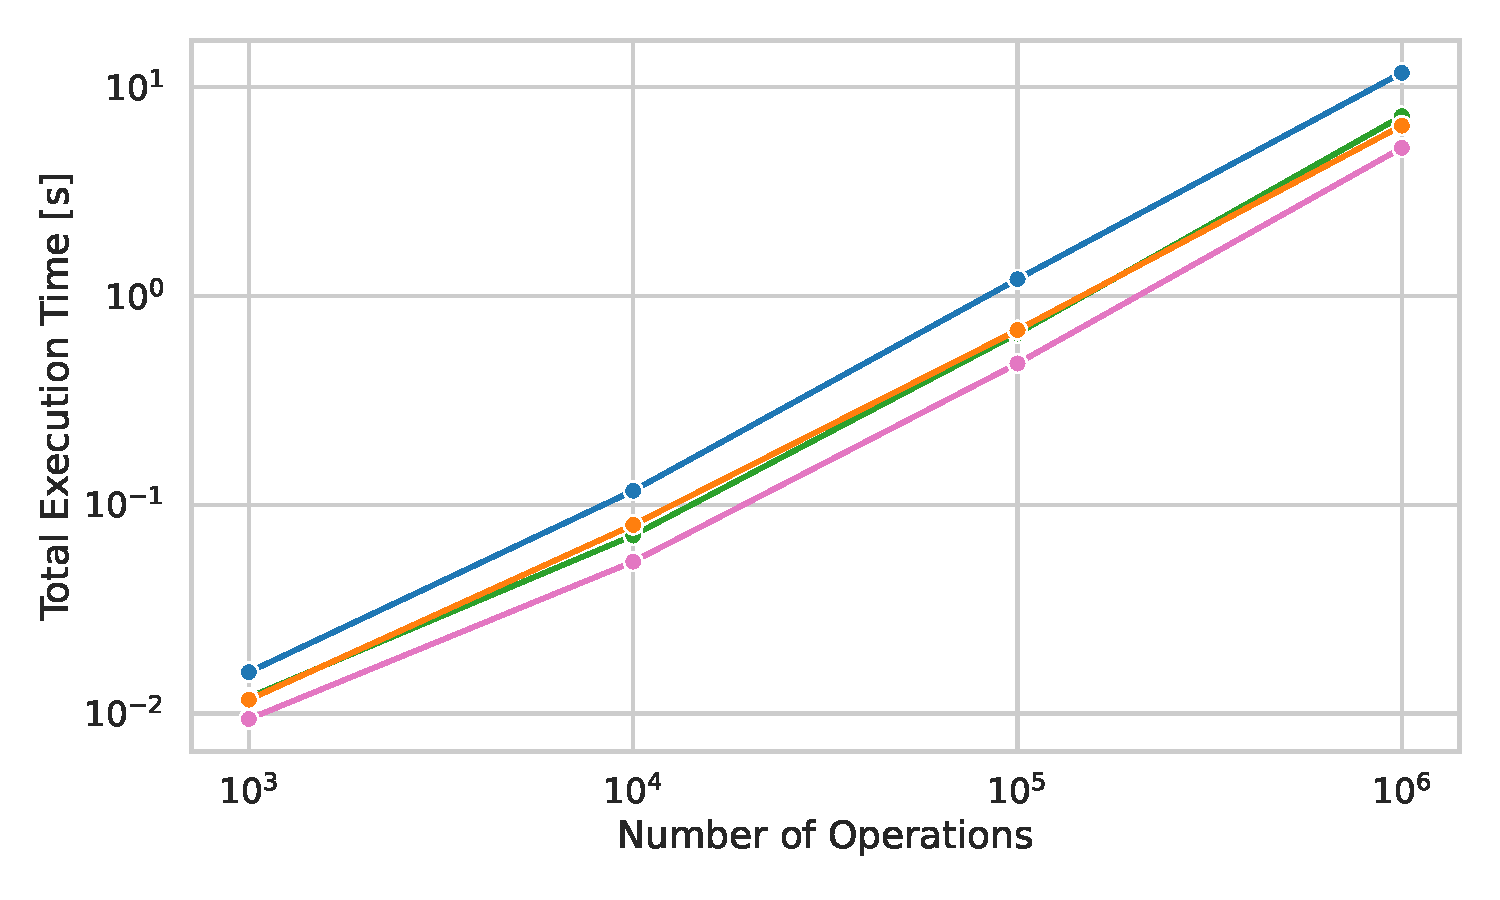
\includegraphics[width=1.0\textwidth]{figures/plots/plot_string_performance.pdf}
    \caption{Total execution time vs number of operations on string keys.}
\end{figure}

\begin{table}[ht]
\centering
\begin{tabular}{|l|r|r|r|r|}
\hline
\textbf{File} & \textbf{Weak Heap} & \textbf{Skew Heap} & \textbf{R-p Heap} & \textbf{STL} \\
\hline
USA-road-d.NY.gr   & 0.0578 & 0.0323 & 0.1410 & 0.0335 \\
USA-road-d.FLA.gr  & 0.2369 & 0.1402 & 0.5291 & 0.1427 \\
USA-road-d.CAL.gr  & 0.4981 & 0.2951 & 0.9647 & 0.3153 \\
USA-road-d.W.gr    & 1.6977 & 1.0162 & 3.2455 & 1.1301 \\
USA-road-d.CTR.gr  & 5.7985 & 4.5255 & 10.0441 & 4.3664 \\
USA-road-d.USA.gr  & 7.0490 & 4.3979 & 13.3550 & 4.6924 \\
\hline
\end{tabular}
\caption{Benchmark results for general-purpose priority queues running Dijkstra's algorithm on USA road network graphs. Times are given in seconds. R-p heap denotes \texttt{RankPairingHeap}. STL denotes \texttt{std::priority\_queue}.}
\label{tab:dijkstra_results}
\end{table}

\subsection{Summary}

The tests allow us to draw several interesting conclusions about the performance of different priority queue implementations. Perhaps the most notable, though expected, result is the very high memory usage of the van Emde Boas priority queue for large universe sizes, as illustrated in Figure~\ref{fig:vEB_memory}. Aside from this, the van Emde Boas priority queue outperforms other integer priority queues, since the constant factors in the implementations of X-fast and Y-fast tries significantly reduce their practical efficiency. This is especially evident in Figure~\ref{fig:Xfast_Yfast_performance}, where those priority queues perform the worst on large sets of random operations.

Among general-purpose priority queues, weak heaps emerge as a viable alternative to the standard binary heap, with performance closely matching the STL priority queue in many test cases. The skew heap, while slightly less efficient on artificial benchmarks, performs exceptionally well on real-world data, outperforming the STL priority queue on all but one test file when used in Dijkstra’s algorithm, as shown in Table~\ref{tab:dijkstra_results}. Conversely, the rank-pairing heap is the least performant among general-purpose priority queues in many cases, likely due to the implementation complexity and the resulting constant-factor overhead.
